\documentclass[a4paper, utf8]{ctexart}
\usepackage[fontset=Fandol]{ctex}
\usepackage{anyfontsize}
\usepackage{algorithm}
\usepackage{longtable}
\usepackage{abstract}
\usepackage{amsfonts}
\usepackage{appendix}
\usepackage{booktabs}
\usepackage{enumitem}
\usepackage{fancyhdr}
\usepackage{geometry}
\usepackage{graphicx}
\usepackage{tabularx}
\usepackage{listings}
\usepackage{amsmath}
\usepackage{caption}
\usepackage{lipsum}
\usepackage{minted}
\usepackage{xcolor}
\usepackage{array}

\geometry{a4paper,left=31mm,right=31mm,top=25mm,bottom=25mm}
\CTEXsetup[format={\Large \bfseries}]{section}

\setlength{\parindent}{2em}
\pagestyle{fancy}
\fancyhf{}
\fancyhead[L]{并行程序设计与算法实验\ 实验报告}
\fancyhead[R]{Lab4\ Pthreads并行方程求解及蒙特卡洛}
\fancyhead[C]{}
\fancyfoot[C]{\thepage}
\fancyfoot[L,R]{}

\setCJKfamilyfont{zhsong}[AutoFakeBold = {2.17}]{SimSun}
\renewcommand*{\songti}{\CJKfamily{zhsong}}
\definecolor{LightGray}{gray}{0.9}

\title{\songti \bfseries Lab4\ Pthreads并行方程求解及蒙特卡洛}
\author{\fangsong 21307210\ \ 傅祉珏}
\date{\fangsong 中山大学计算机学院\ 广东广州\ 510006}

\begin{document}
	
	\begin{titlepage}
		\centering
		\rule{\textwidth}{1pt}
		\vspace{0.02\textheight}
		
		{\LARGE \kaishu 并行程序设计与算法实验\ 实验报告}
		
		\vspace{0.02\textheight}
		
		{\Huge \songti \bfseries Lab4\ Pthreads并行方程求解及蒙特卡洛}
		
		\vspace{0.025\textheight}
		\rule{0.83\textwidth}{0.4pt}
		\vspace{0.05\textheight} 
		\begin{figure}[htbp]
			\centering
			
\includegraphics[width=8cm, height=8cm]{./figure/计院院徽.jpg}
		\end{figure}
		
		\vspace{0.04\textheight} 
		{\Large 姓名:傅祉珏}
		
		\vspace{0.025\textheight} 
		{\Large 学号:21307210}
		
		\vspace{0.025\textheight} 
		{\Large 专业:计算机科学与技术}
		
		\vspace{0.025\textheight} 
		{\Large Email:futk@mail2.sysu.edu.cn}
		
		\vspace{0.025\textheight} 
		{\Large 完成时间:\today}
		
		\vspace{0.05\textheight} 
		\vfill
		
		{\large \today}
		\vspace{0.1\textheight}
		\rule{\textwidth}{1pt}
	\end{titlepage}
	\let\cleardoublepage\clearpage
	
	\maketitle
	
	\renewcommand{\abstractname}{\large \textbf{摘要}}
	\begin{abstract}
		本实验围绕 Pthreads 多线程编程,开展了两项典型并行计算任务:一元二次方程组的批量求解与圆周率 $\pi$ 的蒙特卡洛估算。通过设计细粒度与粗粒度的线程划分策略,实验分别实现了对单个方程计算步骤的线程级并行与对大规模方程集合的多线程批处理,分析了线程同步机制、负载均衡与调度策略对性能的影响。在蒙特卡洛部分,实验通过多线程并行生成随机采样点,并结合点分布统计估算 $\pi$ 值,比较不同线程与样本规模下的估算精度与运行效率。实验结果表明,合理的并行划分与线程调度能显著提升数值计算任务的执行性能,同时展示了多线程模型在处理独立、密集型计算问题中的优势与挑战。通过本实验,深入理解了并发编程在科学计算中的应用潜力与优化思路。
		
		\noindent{\textbf{\heiti 关键词:}Pthreads,多线程并行,一元二次方程,蒙特卡洛方法,性能分析。}
	\end{abstract}
	
	\section{实验目的}
	
	本实验旨在通过基于 Pthreads 线程库的并行程序设计与实现,掌握多线程在数值计算任务中的应用方法,理解线程并发带来的性能优化效果与潜在开销。实验内容主要包括两个典型任务:并行求解一元二次方程组与并行估算圆周率$\pi$值。通过不同线程数量和输入规模下的实验运行,观测程序执行时间与计算精度的变化,系统性地分析多线程并行处理在不同计算模型中的适用性和扩展性。
	
	在一元二次方程求解部分,实验通过将求根公式的各计算步骤细化并划分至多个线程,利用条件变量实现线程间的同步与数据共享,以并行方式加速对多个方程根的求解过程。实验将比较串行与并行实现之间在相同数据集上的执行性能差异,深入探讨线程划分粒度、任务依赖性及线程调度策略对整体效率的影响,增强对线程协作机制与并发控制的理解。
	
	在蒙特卡洛方法估算圆周率部分,实验通过多线程并行生成大量随机采样点,并统计其在单位圆内的分布比例,以此近似计算$\pi$值。实验过程中将测试不同采样点数量与线程数量下的计算时间和结果误差,同时结合图形可视化展示采样点分布与$\pi$值收敛趋势,从而理解蒙特卡洛方法在高性能计算中的并行适应性及其收敛特性。
	
	\section{实验过程}
	
	\subsection{一元二次方程求解}
	
	在本实验的一元二次方程求解部分,我们通过使用 Pthreads 实现了串行与并行两种模式下的大规模方程求解,并对其性能进行了系统测试与比较。实验首先构建了包含 500,000 个一元二次方程的数据集,每个方程的系数$a,b,c$由随机函数生成,确保测试数据的多样性和复杂性。
	
	实验首先实现了传统串行求解的方式,利用判别式$\Delta=b^2-4ac$判断方程根的存在性,并使用求根公式分别计算两个实数根。在对比性能时,先对单个方程进行求解并记录时间,然后扩展到对整个数据集的串行处理过程,统计500,000个方程全部求解所需的总时间,为后续的并行优化提供基准参考。
	
	\begin{minted}[baselinestretch=1, framesep=0mm, escapeinside=||]{cpp}
void solve_serial_single(double a, double b, double c, double* x1, double* x2) {
    double delta = b * b - 4 * a * c;
    if (delta < 0 || a == 0) {
        *x1 = *x2 = NAN;
    } else {
        double sqrt_delta = sqrt(delta);
        *x1 = (-b + sqrt_delta) / (2 * a);
        *x2 = (-b - sqrt_delta) / (2 * a);
    }
}
	\end{minted}
	
	接着,我们设计并实现了两种并行方案。一种是针对单个方程的细粒度并行计算,通过三个线程分别负责计算判别式、开平方、以及根的求解。线程之间通过互斥锁(\verb|pthread_mutex_t|)和条件变量(\verb|pthread_cond_t|)实现同步,确保数据依赖关系的正确性。此方法验证了在细粒度任务中,线程同步机制的实际表现和开销情况,并通过时间对比展示了多线程是否能在轻量任务中带来加速效果。
	
	\begin{minted}[baselinestretch=1, framesep=0mm, escapeinside=||]{cpp}
void solve_parallel_single(double in_a, double in_b, double in_c, double* out_x1,
                           double* out_x2) {
    a = in_a;
    b = in_b;
    c = in_c;
    delta_ready = sqrt_ready = 0;

    pthread_t t1, t2, t3;
    pthread_create(&t1, NULL, compute_delta, NULL);
    pthread_create(&t2, NULL, compute_sqrt_delta, NULL);
    pthread_create(&t3, NULL, compute_roots, NULL);
    pthread_join(t1, NULL);
    pthread_join(t2, NULL);
    pthread_join(t3, NULL);

    *out_x1 = x1;
    *out_x2 = x2;
}
	\end{minted}
	
	另一种更具代表性的并行方案是针对大批量方程的并行求解。我们将整个数据集均匀分配给8个线程,每个线程处理不同编号的方程,从而最大限度地利用多核处理器的计算能力。该方法避免了线程之间的通信与同步开销,使得各线程可以独立高效地完成任务。通过对并行处理所用总时间的测量,我们观察到了显著的运行时间下降,验证了任务划分与负载均衡在并行计算中的关键作用。
	
	\begin{minted}[baselinestretch=1, framesep=0mm, escapeinside=||]{cpp}
void* batch_worker(void* arg) {
    int tid = *(int*)arg;
    for (int i = tid; i < N; i += NUM_WORKERS) {
        Equation* eq = &equations[i];
        double d = eq->b * eq->b - 4 * eq->a * eq->c;
        if (d < 0 || eq->a == 0) {
            eq->x1 = eq->x2 = NAN;
        } else {
            double s = sqrt(d);
            eq->x1 = (-eq->b + s) / (2 * eq->a);
            eq->x2 = (-eq->b - s) / (2 * eq->a);
        }
    }
    return NULL;
}

void solve_parallel_batch() {
    pthread_t threads[NUM_WORKERS];
    int ids[NUM_WORKERS];
    for (int i = 0; i < NUM_WORKERS; ++i) {
        ids[i] = i;
        pthread_create(&threads[i], NULL, batch_worker, &ids[i]);
    }
    for (int i = 0; i < NUM_WORKERS; ++i) {
        pthread_join(threads[i], NULL);
    }
}
	\end{minted}
	
	综合实验过程可见,从单个方程的细粒度并行,到大规模数据的粗粒度并行处理,线程创建、任务划分和同步机制的选择对程序性能具有直接影响。本实验不仅加深了我们对一元二次方程求解过程的理解,更使我们掌握了如何结合具体问题特性灵活设计并行策略,从而提升整体计算效率。
	
	\subsection{蒙特卡洛方法求$\pi$的近似值}
	
	在本实验的蒙特卡洛方法求$\pi$的近似值部分,我们通过使用 Pthreads 实现了并行计算策略,并对比了不同采样点数和线程数下的性能表现与估算精度。实验的目标是通过在单位正方形内随机生成点,利用点落在单位圆内的比例来估算圆周率 $\pi$ 的值。我们设计了一种基于线程的并行计算方法,以加速大量采样点的处理过程。
	
	首先,我们为实验构建了一个动态变化的点集,点的数量从最小的1024个增加到最大65536个,步长为1024。在每个实验中,我们将总点数均匀地分配给8个线程,每个线程独立生成随机点,并判断这些点是否位于单位圆内。每个线程通过独立的种子生成随机数,避免了线程之间的种子冲突,确保每个线程的随机性。
	
	在实验中,首先实现了串行计算模式,即单线程处理所有点的生成与计算。通过这种方式,我们能够得到一个基准性能,记录单线程在不同点数下的运行时间和估算结果。之后,我们通过 Pthreads 实现了并行版本的蒙特卡洛计算。每个线程负责计算一部分随机点,并统计其中位于单位圆内的点数。所有线程计算完成后,主线程将结果合并,并根据总的圆内点数计算 $\pi$ 的近似值。
	
	\begin{minted}[baselinestretch=1, framesep=0mm, escapeinside=||]{cpp}
void* monte_carlo_worker(void* arg) {
    ThreadData* data = (ThreadData*)arg;
    long in_circle = 0;
    for (long i = 0; i < data->points_per_thread; ++i) {
        double x = rand_r(&data->seed) / (double)RAND_MAX;
        double y = rand_r(&data->seed) / (double)RAND_MAX;
        if (x * x + y * y <= 1.0)
            in_circle++;
    }
    data->points_in_circle = in_circle;
    return NULL;
}
	\end{minted}
	
	我们对每次实验都记录了总点数、圆内点数、估算出的 $\pi$ 值以及运行时间,并将这些数据保存到 \verb|pi_estimates.csv| 文件中,便于后续分析。此外,为了直观展示采样点的分布情况,我们在最小和最大点数两个点数规模下保存了所有生成点的位置数据,并分类标记为圆内或圆外,保存为 \verb|points_plot_data.txt|,可以用于生成散点图进行结果可视化。
	
	\section{实验结果}
	
	\subsection{一元二次方程求解}
	
	在一元二次方程求解的实验中,我们分别对串行与并行两种求解策略在不同数据规模下的运行时间进行了量化比较。通过构造从 1 个方程至 500,000 个方程的数据集,并测量每种方案在相应任务规模下的执行时间,我们可以清晰地观察线程并行带来的性能变化和提升趋势。
	
	首先,在串行运行的测试中,随着待求解方程数量的增长,运行时间整体呈上升趋势。尤其在方程数量达到 500,000 时,平均运行时间达到了 5185.60 纳秒。尽管中间存在一定波动(如在 250,000 个方程时下降到约 3016 纳秒),但整体呈现线性增长趋势,符合串行计算复杂度随任务量线性增加的预期。
	
	相比之下,Pthreads 实现的并行求解方式在大多数数据规模下都表现出显著优于串行的计算效率。例如,在 500,000 个方程时,并行平均运行时间为 2996.96 纳秒,相比串行减少了 约42\%。而在中等规模(如 150,000 个方程)下,并行平均时间为 1206.56 纳秒,同样显著优于串行的 2010.95 纳秒。尤其值得注意的是,在数据规模相对较小(如 100,000 个方程)时,并行时间甚至低至 1146.50 纳秒,表明多线程的划分与调度开销并未对总体性能造成太大负担。
	
	不过,在数据规模较小时(如 1 个方程的测试),并行计算并未体现出优势,反而因线程创建及调度开销使运行时间升高至 331.86 纳秒,明显高于串行的 0.27 纳秒。这也验证了多线程机制在细粒度计算任务中易受到线程管理开销影响,从而无法实现性能提升。
	
	总体来看,实验结果清楚表明,在大规模任务场景中,采用 Pthreads 进行任务划分与并行求解可有效提升整体计算效率,尤其适用于方程数量达到数十万量级以上的情况。而在任务规模较小时,串行解法仍具有轻量、高效的优势。因此,合理选择求解策略应基于任务规模、线程数及调度成本等因素进行权衡,从而实现性能与资源利用的最佳平衡。
	
	\begin{figure}
		\centering
		\begin{minipage}{.45\textwidth}
			\centering
			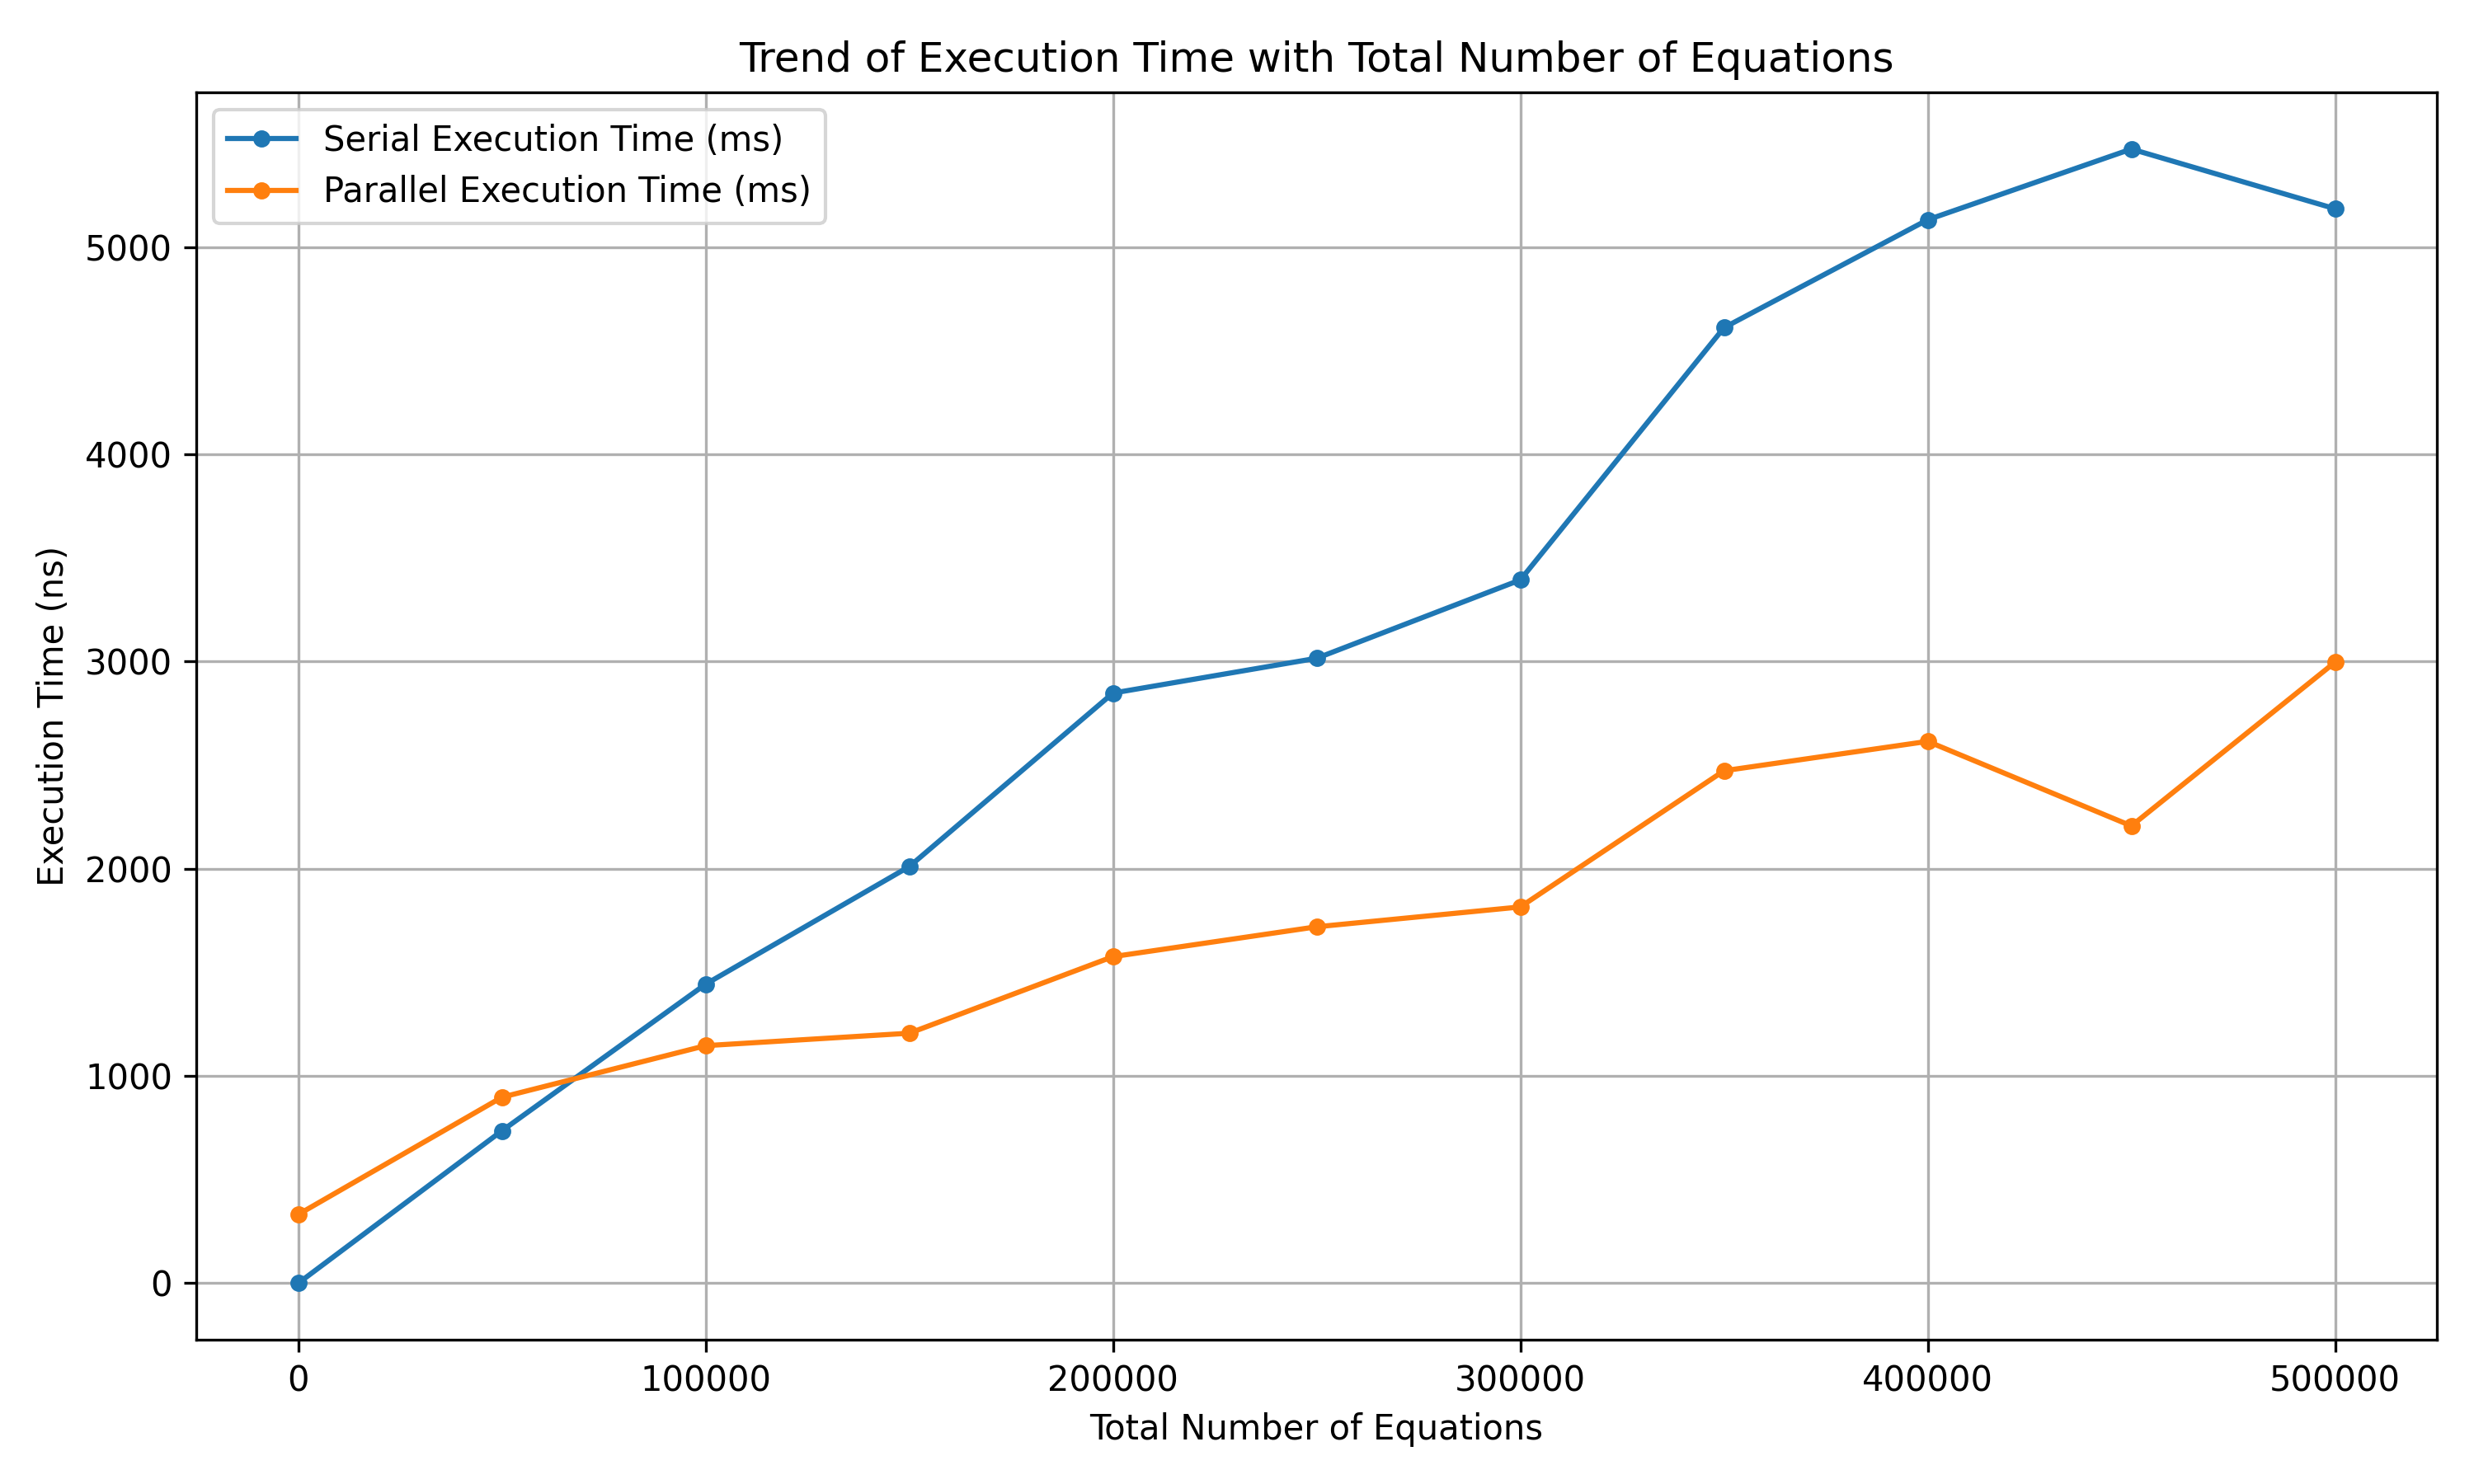
\includegraphics[width=.8\textwidth]{./figure/time_trend.png}
			\caption{一元二次方程求解运行性能趋势图}
		\end{minipage}
		\begin{minipage}{.45\textwidth}
			\centering
			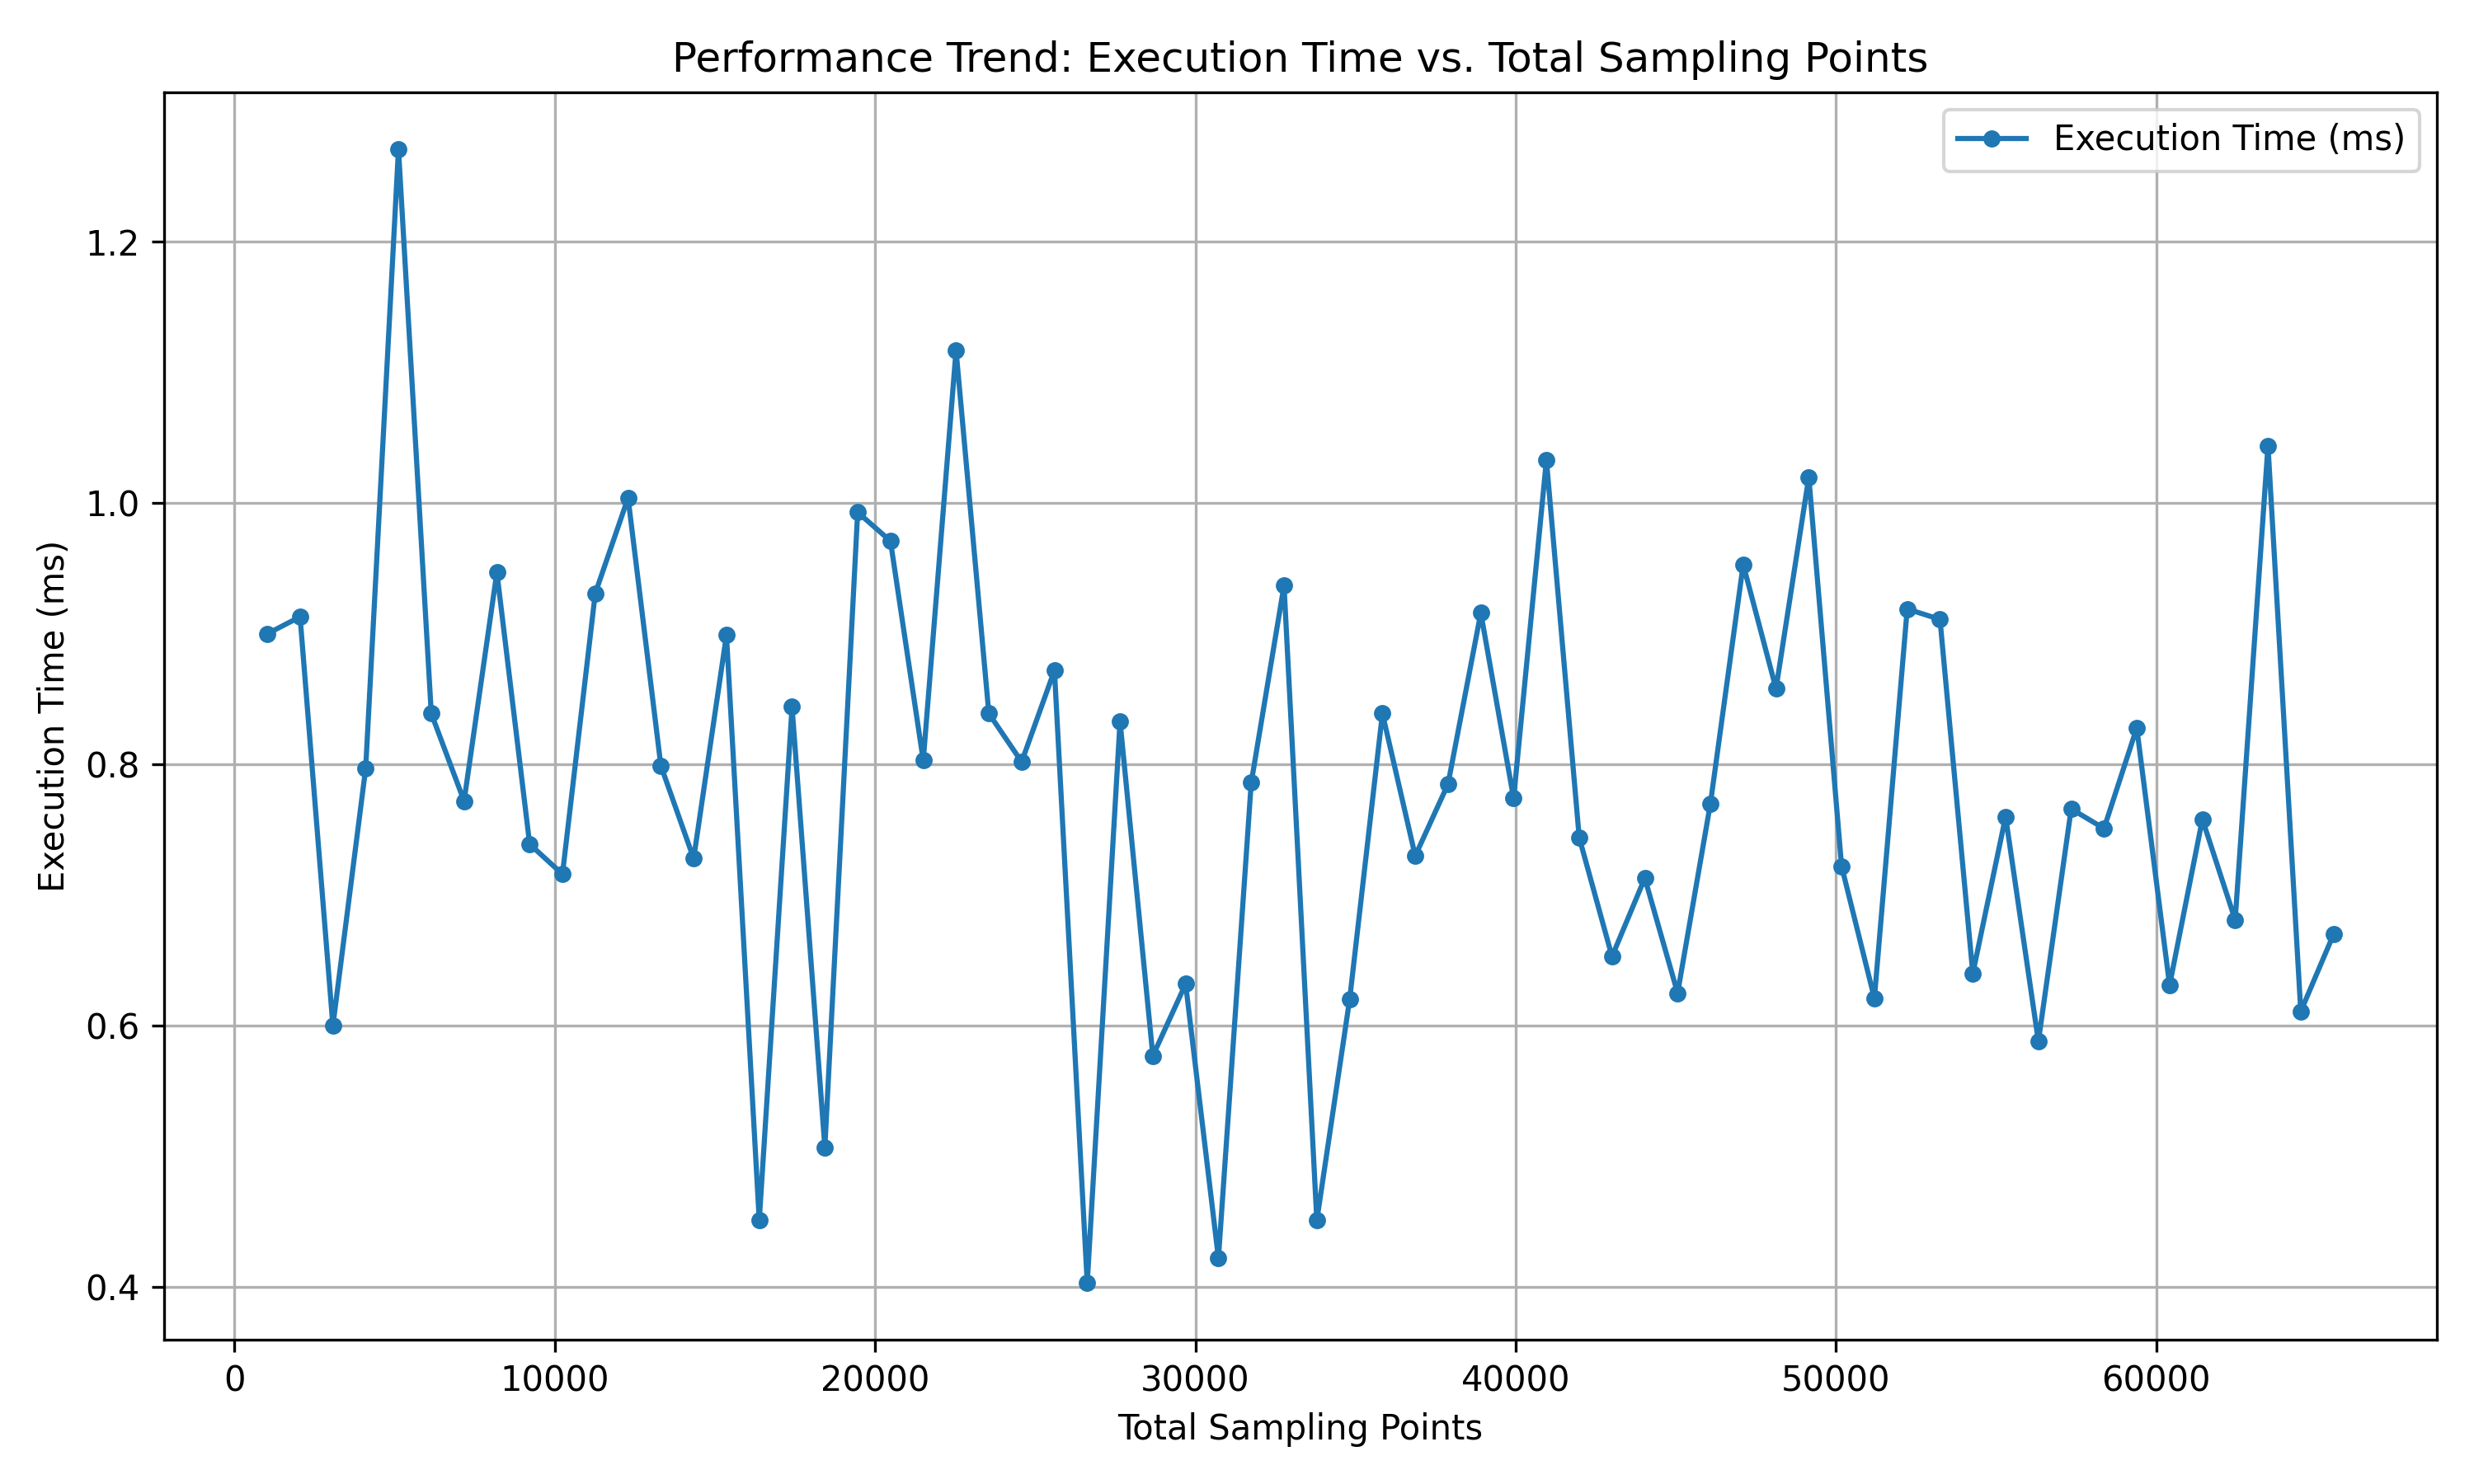
\includegraphics[width=.8\textwidth]{./figure/performance_trend.png}
			\caption{蒙特卡洛求$\pi$运行性能趋势图}
		\end{minipage}
	\end{figure}
	
	\subsection{蒙特卡洛方法求$\pi$的近似值}
	
	在本次实验中,我们采用蒙特卡洛方法通过抛点法随机估计圆周率 $\pi$ 的近似值,并结合 Pthreads 实现对大量样本点的并行处理。实验通过逐步增加总投点数量,从 1024 增加至 65536,并记录每个样本点数量下落入单位圆内的点数、估算出的 $\pi$ 值及对应运行时间。
	
	从结果数据来看,随着投点总数的逐步提升,所估算的 $\pi$ 值逐渐趋近于数学常数 $\pi \approx 3.14159265$,且波动范围逐步减小。例如在投点数量为 1024 时,估算值为 3.1289,与真实值存在一定偏差;而在投点数量达到 65536 时,估算值为 3.14276,已非常接近真实值,说明样本量越大,估计值越趋于稳定,符合蒙特卡洛法的基本统计特性。同时,估计结果总体分布于 $[3.12, 3.17]$ 区间内,波动较小,验证了方法的有效性与合理性。
	
	在性能方面,多线程的使用显著提升了整体运行效率。在不同样本规模下,程序的运行时间基本保持在 1 毫秒以内,大部分数据点的耗时集中在 0.6 到 0.9 毫秒之间,甚至在某些规模较大的样本点数量(如 26624、30720)下也可稳定控制在 0.4 毫秒左右,展现出良好的并行性能与计算稳定性。这表明 Pthreads 能有效地对抛点任务进行多线程分割与并行计算,使得即使在大规模实验条件下,程序也能在毫秒级别内完成任务。
	
	\begin{figure}
		\centering
		\begin{minipage}{.4\textwidth}
			\centering
			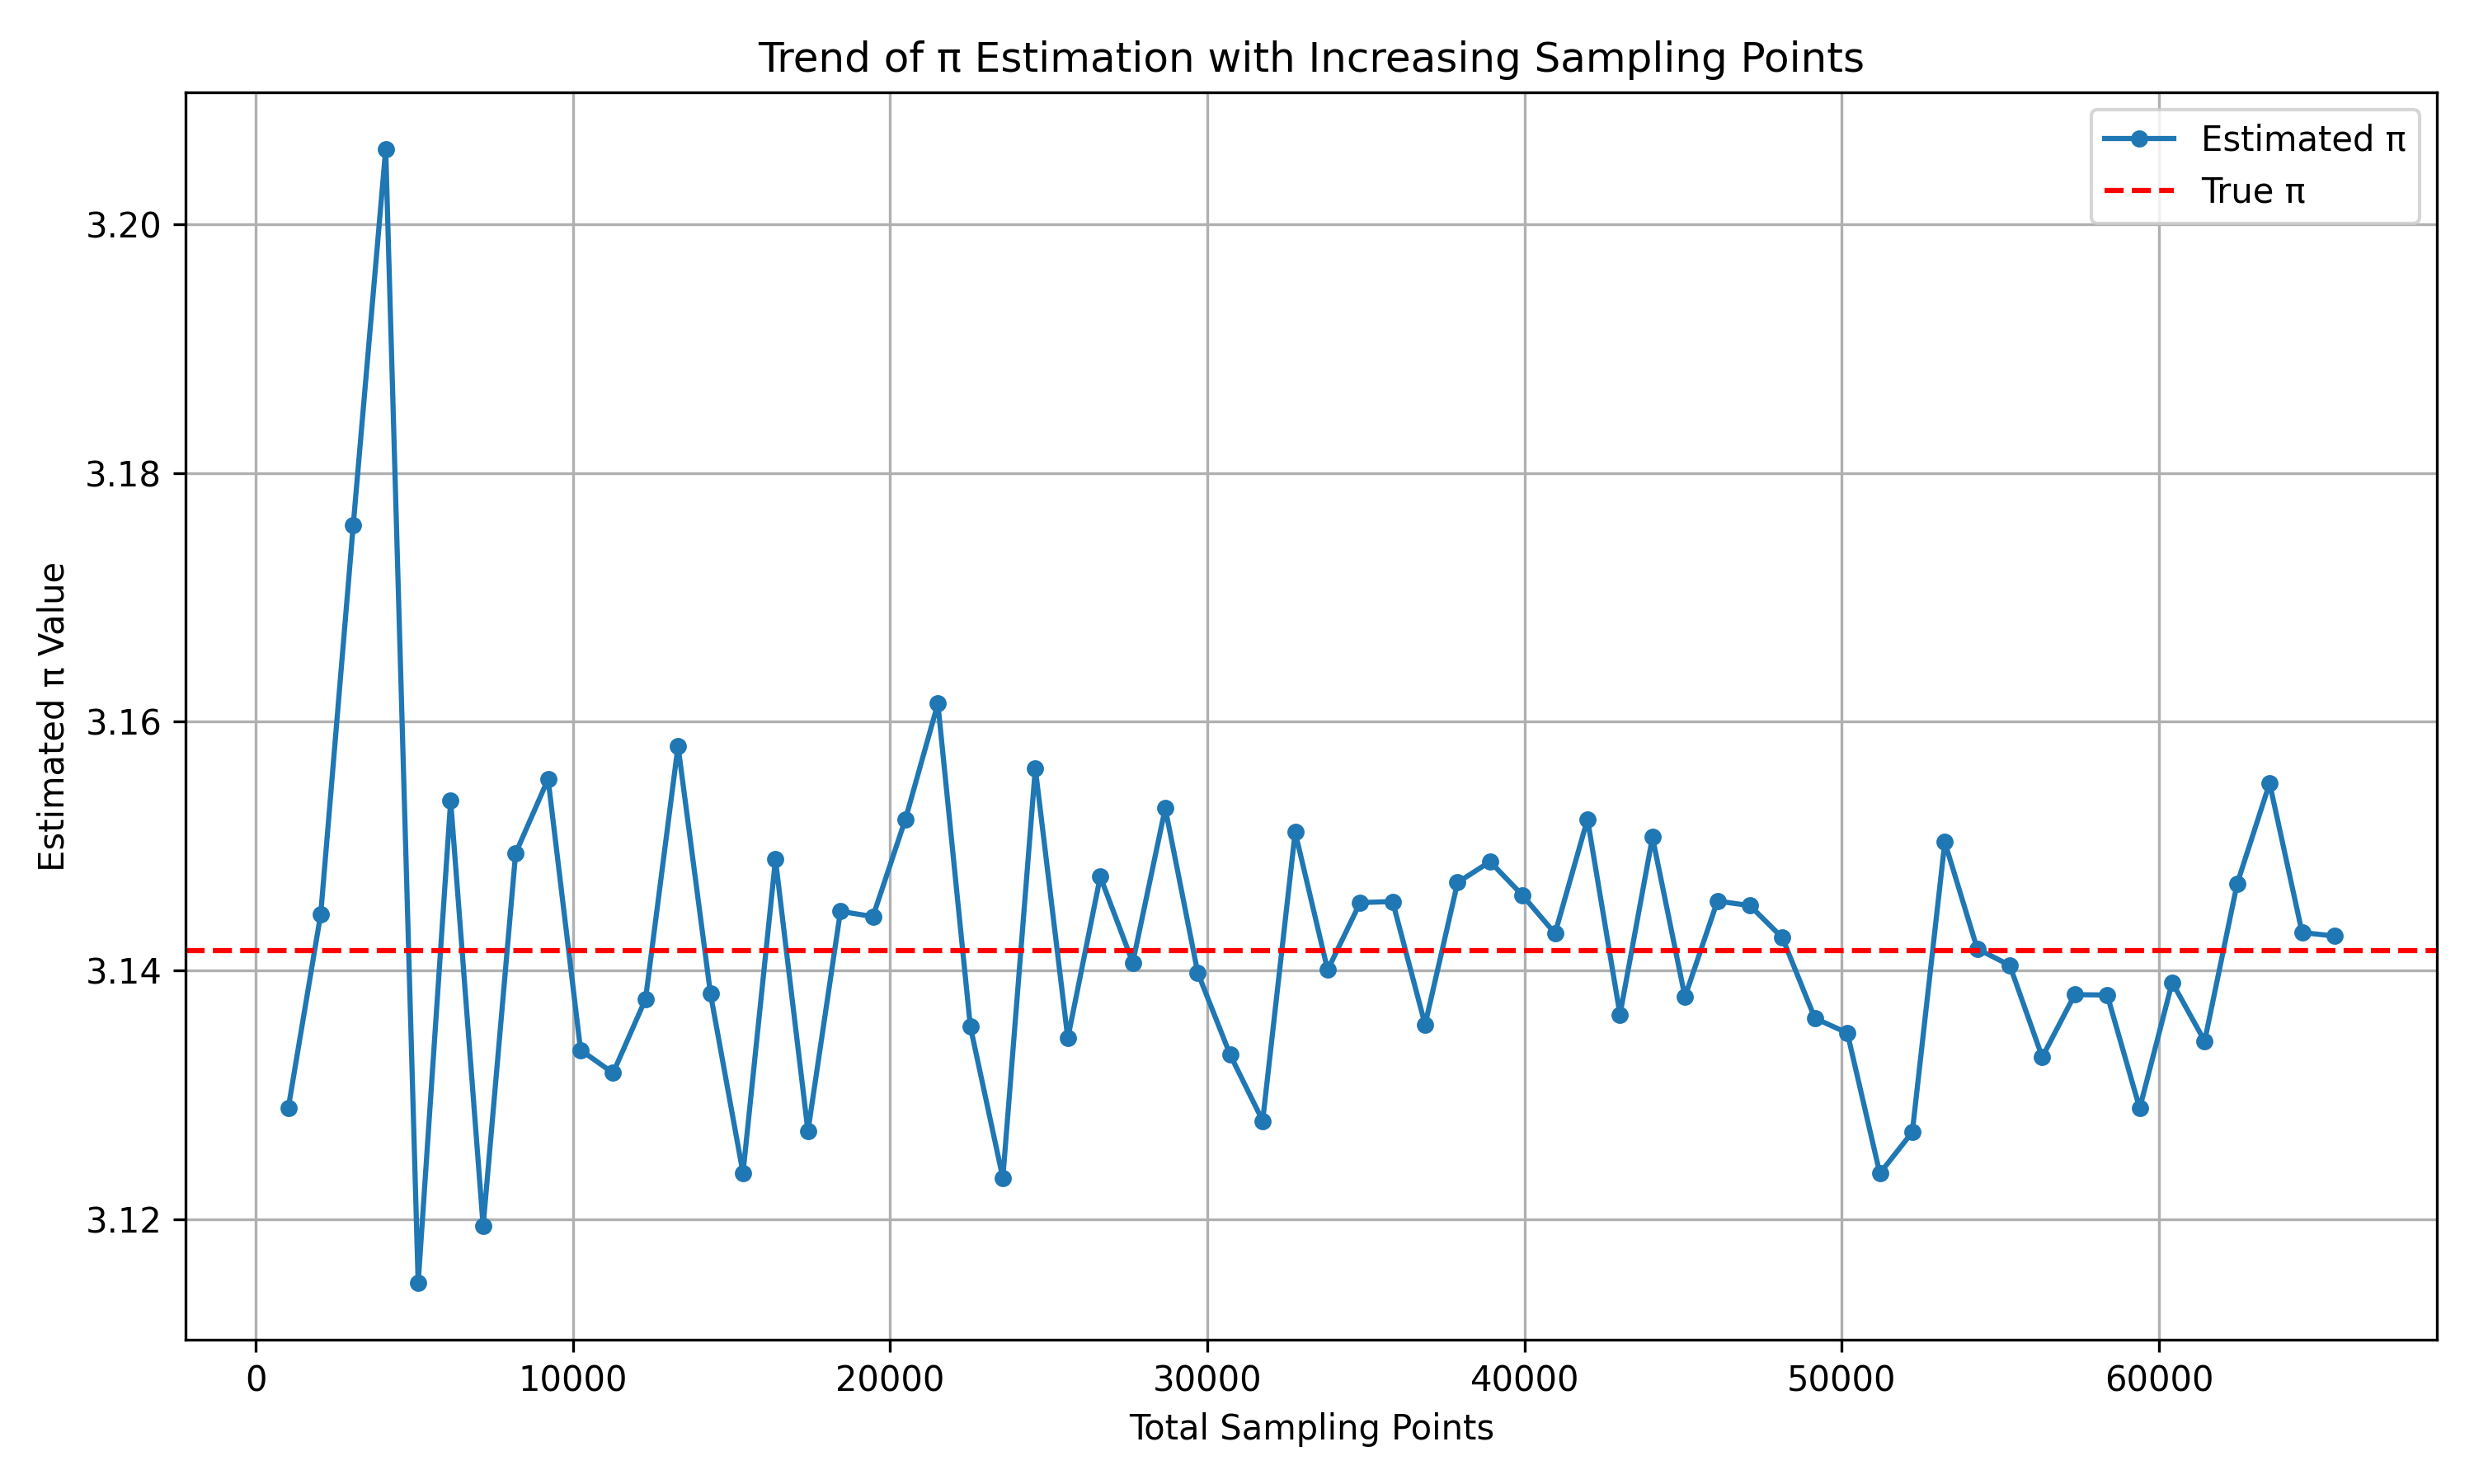
\includegraphics[height=.13\textheight]{./figure/pi_trend.png}
			\caption{$\pi$值趋势图}
		\end{minipage}
		\begin{minipage}{.26\textwidth}
			\centering
			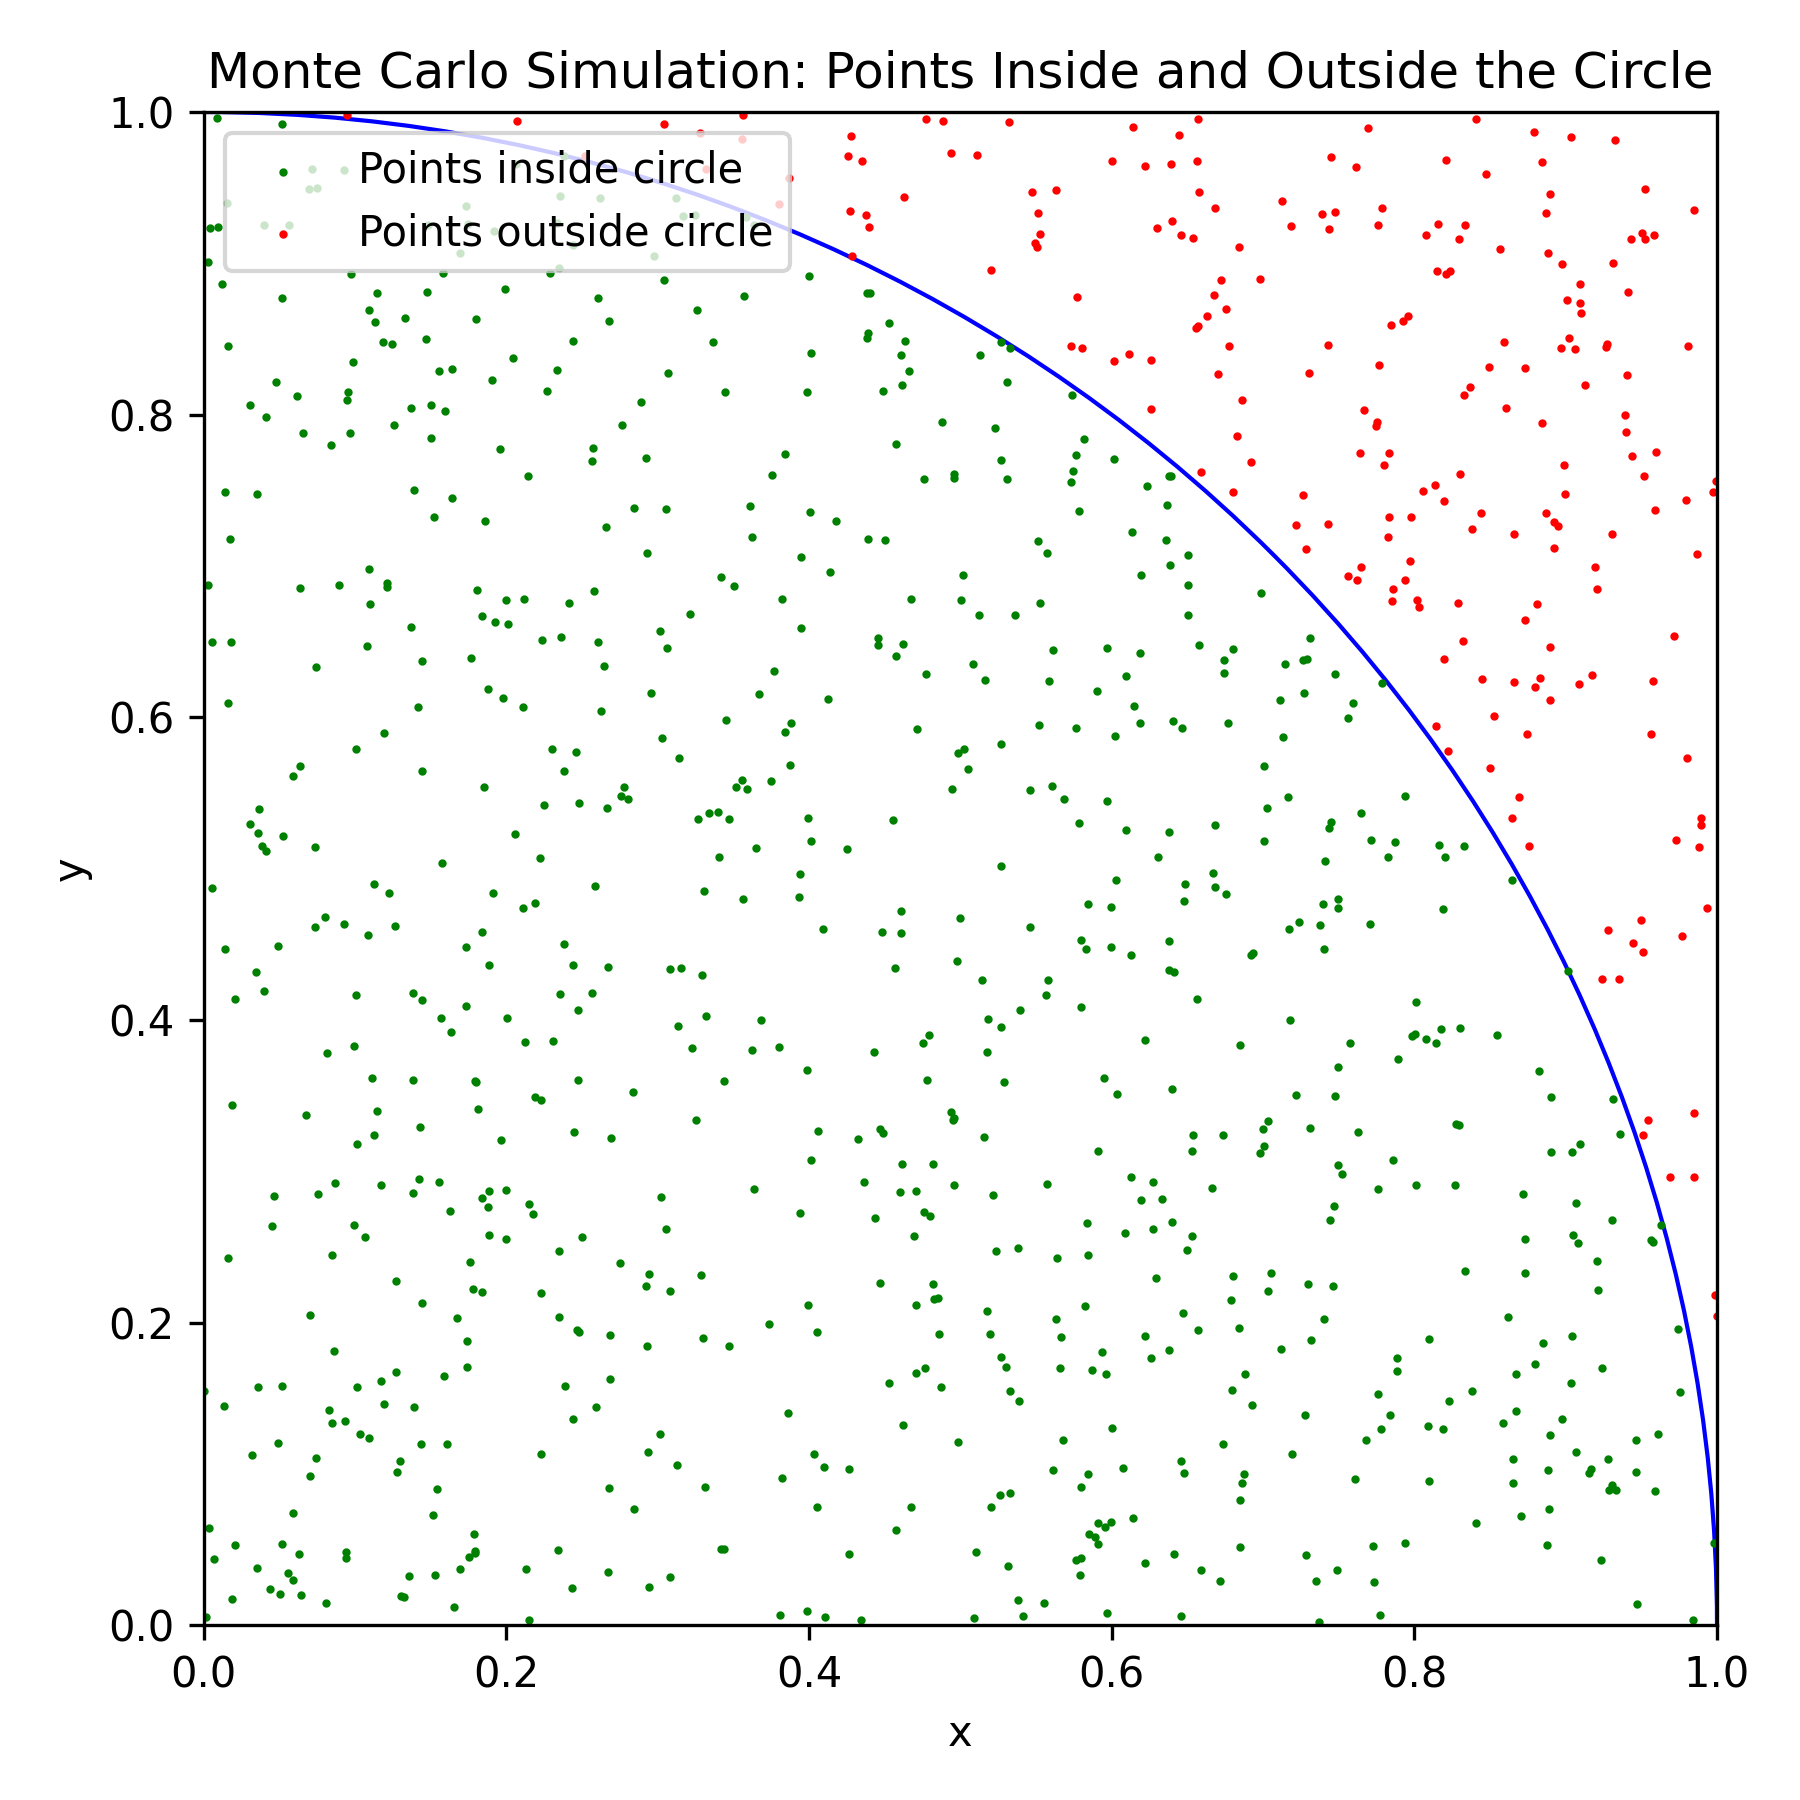
\includegraphics[height=.13\textheight]{./figure/points_plot_1024.png}
			\caption{模拟点图(1024)}
		\end{minipage}
		\begin{minipage}{.26\textwidth}
			\centering
			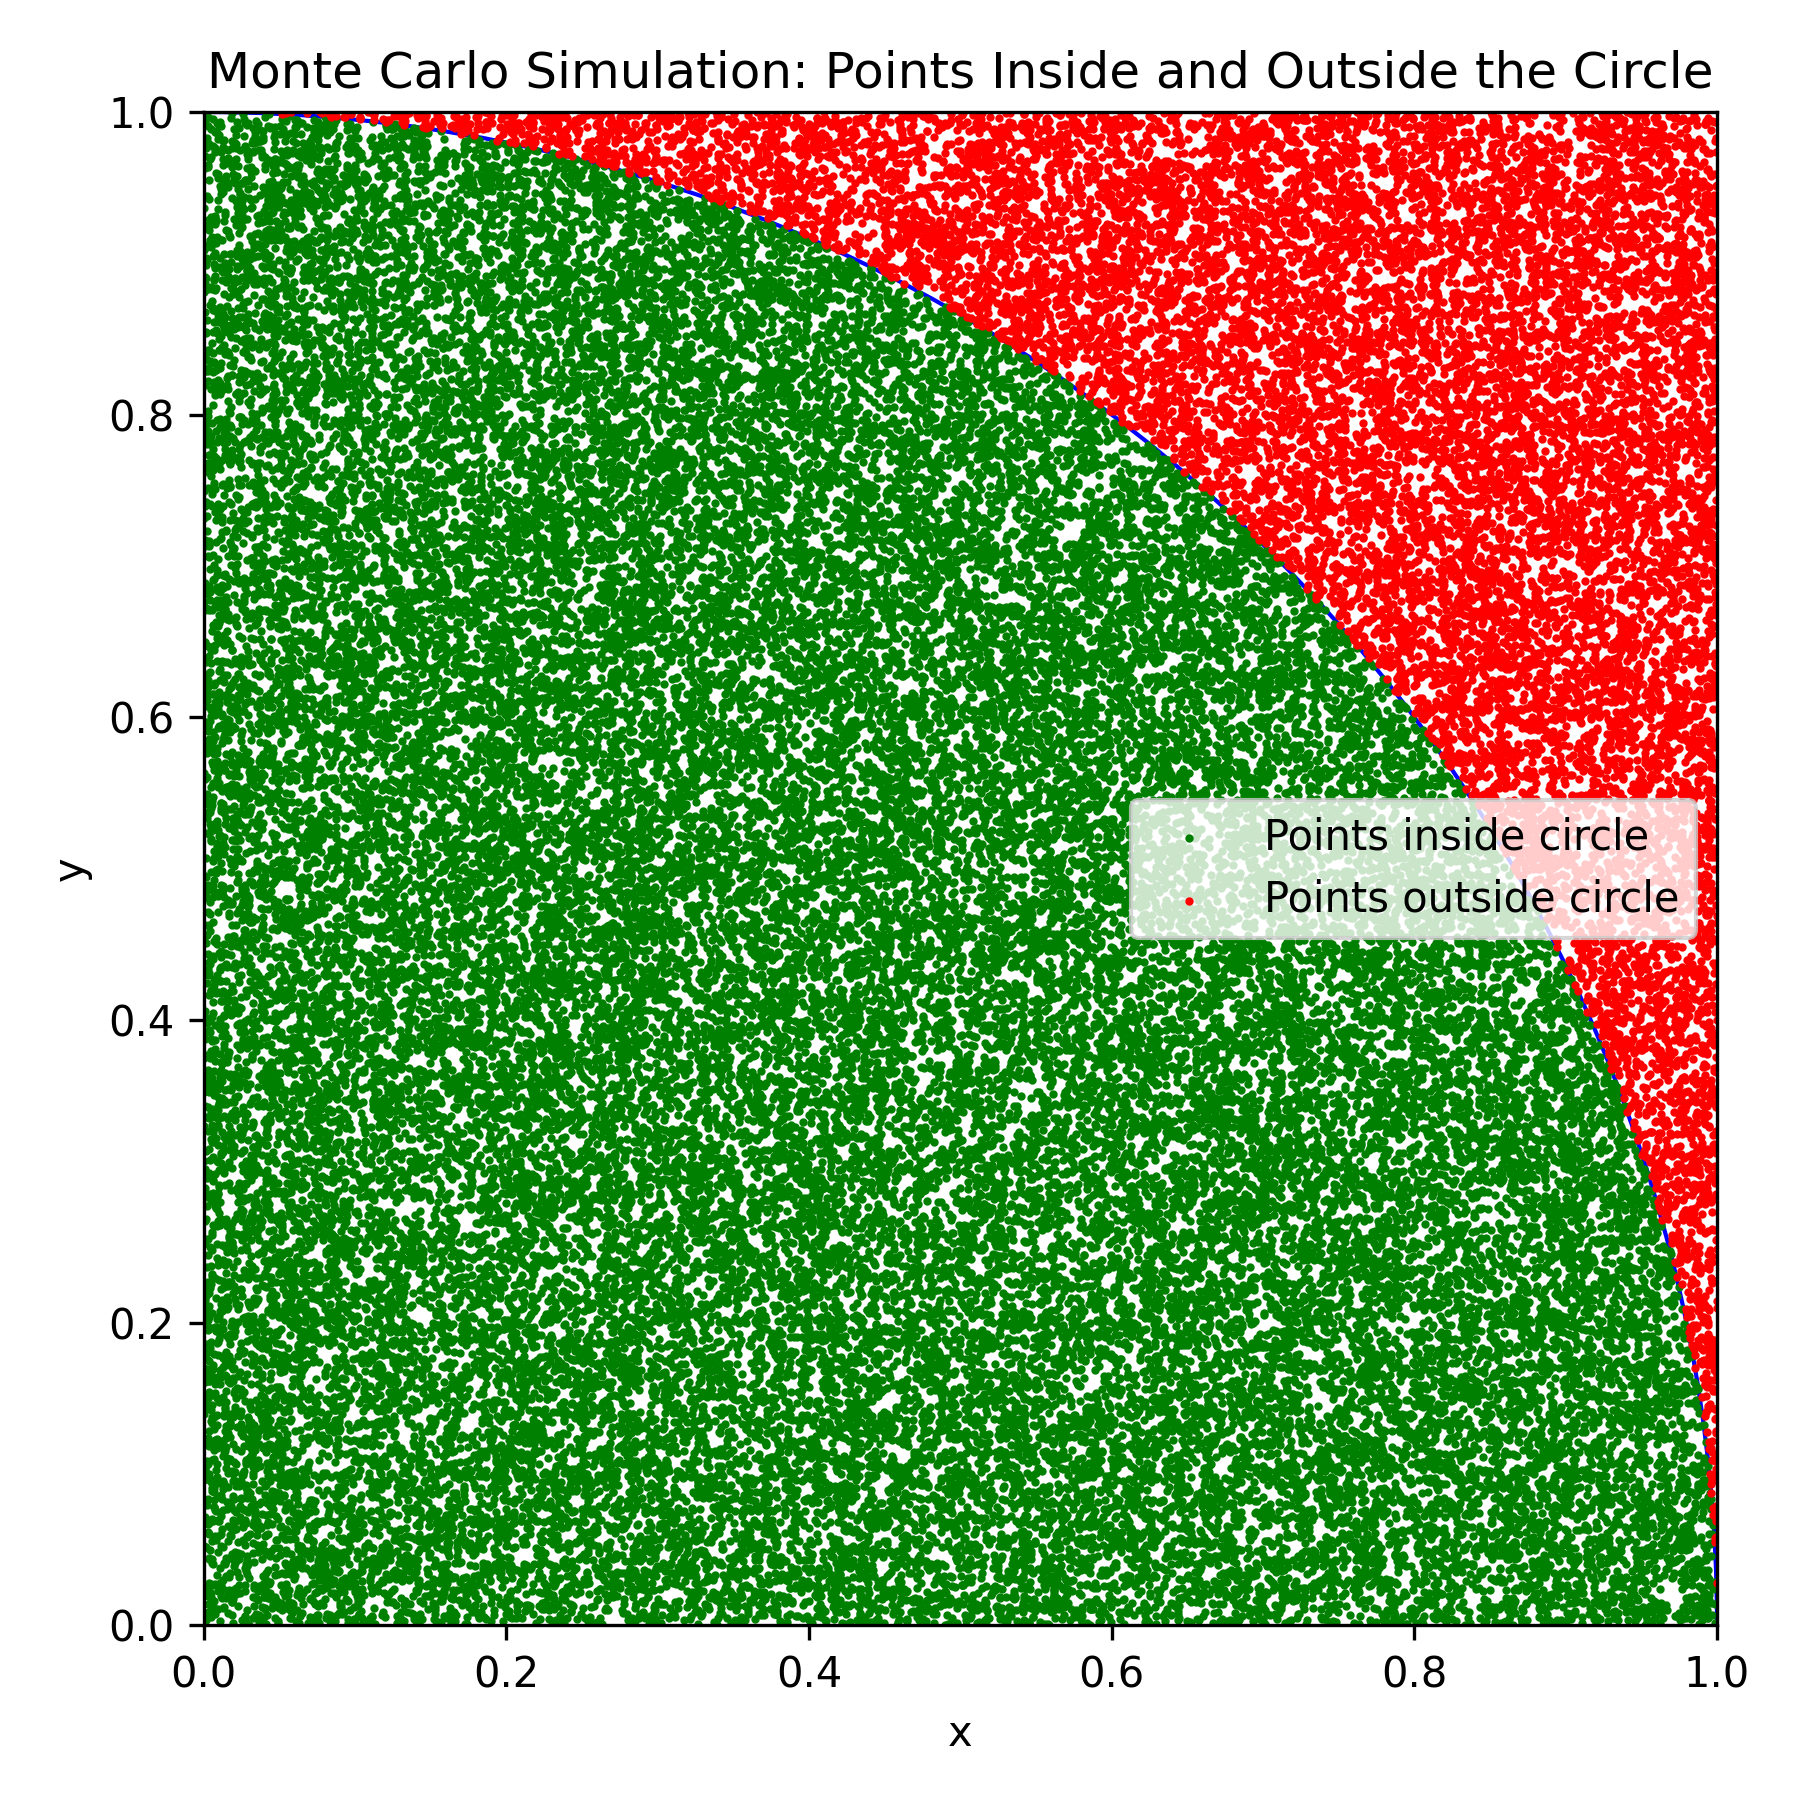
\includegraphics[height=.13\textheight]{./figure/points_plot_65536.png}
			\caption{模拟点图(65536)}
		\end{minipage}
	\end{figure}
	
	综上所述,本实验中蒙特卡洛方法结合 Pthreads 多线程机制,不仅在精度上随着样本数提升而逼近真实值,而且在性能上展现出高度可扩展性与计算效率,充分体现了并行计算在大规模统计模拟中的应用潜力。该实验也直观展示了蒙特卡洛方法在 $\pi$ 值估算等概率问题中的收敛特性与稳定性,为后续更复杂的随机模拟与并行数值方法奠定了良好基础。
	
	\section{总结与思考}
	
	\subsection{实验总结}
	
	本次实验以 Pthreads 多线程机制为核心,围绕两类问题展开:一是对大量一元二次方程的求解,二是基于蒙特卡洛方法估计圆周率 $\pi$。在一元二次方程求解实验中,我们通过对比串行与并行执行效率,观察多线程在不同数据规模下的性能表现。实验结果表明,随着方程数量的增加,并行方法在执行时间上呈现出显著优势,尤其在百万级输入规模下,运行时间明显低于串行实现,体现了线程并发带来的计算加速效应。
	
	在蒙特卡洛估算 $\pi$ 的实验中,我们同样利用多线程将投点任务划分为多个子任务并行执行。通过逐步增加投点数量,我们验证了蒙特卡洛方法的统计收敛性——估算值逐步逼近真实的圆周率,同时保持波动范围可控。配合多线程机制后,即便在高投点数量下,运行时间仍能维持在毫秒级别,展现了 Pthreads 在线程分工与负载均衡方面的高效性。
	
	综上,实验不仅验证了并行编程在数值计算中的加速效果,也在性能测试与实验设计中体现了线程控制、任务划分、收敛性分析等重要并行计算原理,具备良好的实用价值与学习意义。
	
	\subsection{实验心得}
	
	通过本次实验,我深刻体会到了并行计算在提升计算性能方面的巨大潜力。以往在课程中学习线程模型与同步机制时较为抽象,而本实验将这些知识具体化、实践化,使我在编程实践中真正理解了线程创建、任务分配与并行同步的核心逻辑。例如在方程求解任务中,我需要合理划分每个线程的工作区间,处理线程间数据竞争与合理合并结果的问题;而在蒙特卡洛方法中,则进一步体会到并行模式下随机模拟任务的天然适配性,尤其是“数据独立性”在并行划分中的重要意义。
	
	此外,在分析实验数据时,我也意识到性能提升并非完全线性受益,线程管理开销与任务划分策略会直接影响最终效率,因此仅有并行并不够,合理的并行策略同样关键。此次实验让我对“如何设计高效的多线程程序”有了更系统的思考,也增强了我对多核并行计算环境下资源利用与负载优化的敏感性。
	
	总体而言,这次实验不仅是一次编程能力的锻炼,更是对并行计算思想的一次深度实践,加深了我对理论知识与实际应用之间关系的理解,也让我更加期待在后续项目中尝试更复杂的并行编程任务。
	
	\let\cleardoublepage\clearpage
	
	\begin{thebibliography}{99}  
		\bibitem{ref1} 彼得·S·帕切科,\ 马修·马伦塞克.\ 并行程序设计导论[M].\ 黄智濒,\ 肖晨\ 译.\ 原书第2版.\ 北京:机械工业出版社,\ 2024.
		\bibitem{ref2} 黄聃.\ 课件5[EB/OL].\ [2025-3-10].\ https://easyhpc.net/course/221/lesson/1416/material/3173.
	\end{thebibliography}
	
\end{document}
